\documentclass[11pt, a4paper]{article}

\usepackage[margin=3cm, top=2.54cm, bottom=2.54cm]{geometry}

%Font
\usepackage{fontspec}
\setmainfont{Times New Roman}

%Spacing
\renewcommand{\baselinestretch}{1}
\setlength{\textfloatsep}{11pt plus 1pt minus 1pt}
\setlength\abovecaptionskip{0pt plus 1pt minus 1pt}
% \setlength\belowcaptionskip{0pt plus 1pt minus 1pt}

%Write text in math mode
\usepackage{amsmath}
%SI unit
\usepackage{siunitx}

%indent first paragraph
\usepackage{indentfirst}

%lipsum
\usepackage{lipsum}

%Customize section, subsection and subsubsection
\usepackage{titlesec}
\titleformat{\section}[hang]{\centering\large\bfseries}{}{0pt}{}[]
\titlespacing{\section}{0pt}{12pt}{11pt}
\titleformat{\subsection}[hang]{\large\bfseries}{}{0pt}{}[]
\titlespacing{\subsection}{0pt}{11pt}{11pt}
\titleformat{\subsubsection}[hang]{\normalfont}{}{0pt}{}[]
\titlespacing{\subsubsection}{0pt}{11pt}{11pt}


%list
\usepackage{enumitem}

%Caption
\usepackage[labelfont=bf, labelsep=period, justification=centering]{caption}
\usepackage{subcaption}

%Graphics
\usepackage{graphicx}
\usepackage{float}
\graphicspath{{pictures/}}

%Tabel
\usepackage{booktabs}

%Reference & citing
\usepackage{hyperref, letltxmacro}
\usepackage[
    backend=biber,
    style=ieee,
    sorting=ynt,
    isbn=true,
    url=true,
    doi=true
]{biblatex}
\addbibresource{reference.bib}
\usepackage[nameinlink]{cleveref}
\crefname{figure}{Fig.}{Fig.}
\Crefname{figure}{Figure.}{Figure.}

\begin{document}
\begin{center}
    {\textbf{\Large JUDUL JURNAL}}\par
    \vspace{12pt}
    $\text{Penulis pertama}^{1, \dagger},\;\text{Penulis kedua}^1,\;\text{Penulis ketiga}^1,\;\text{Penulis keempat}^1$\par
    \vspace{11pt}
    {\textit{\small \textsuperscript{1}Institusi penulis}}\par
    $^\dagger \text{{\textit{\small Corresponding author: email corresponding author}}}$
\end{center}
\vspace{11pt}
\noindent \textbf{Abstrak.} \lipsum[1]\par
\vspace{11pt}
\noindent \textbf{Kata Kunci:} Arduino Uno, LDR, Laser\par
\vspace{11pt}
\noindent \textit{\textbf{Abtract.} \lipsum[1]}\par
\vspace{11pt}
\noindent \textit{\textbf{Keyword:} Arduino Uno, LDR, Laser}\par

\section{PENDAHULUAN}
\begin{figure}[H]
    \centering
    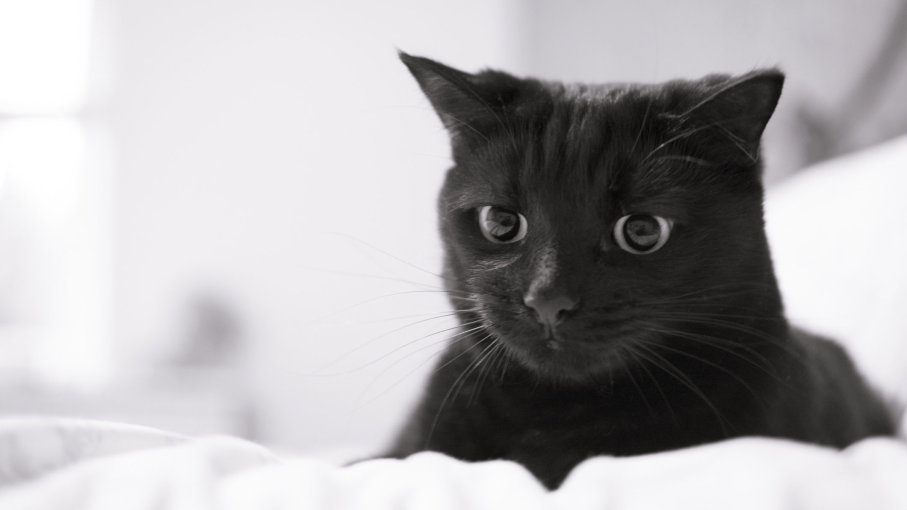
\includegraphics[height=5cm]{random-cat}
    \caption{Picture of random cat found on internet}\label{gambar:random-cat}
\end{figure}
ini~\cref{gambar:random-cat} merupakan contoh referensi.
\lipsum[1]
\section{METODE PEMBUATAN ALAT}
\lipsum[1]
\section{PENGUJIAN DAN ANALISIS}
Bibliography in IEEE style:

Newton's law of universal gravitation states that \textit{each mass particle attracts every other particle in the universe with a force that varies direcly as the product of the two masses and inversely as the square of the distance between them.}~\autocite{book:classical}

\lipsum[1]
\section{KESIMPULAN}
\begin{enumerate}[topsep=0pt,itemsep=-1ex,partopsep=1ex,parsep=1ex, leftmargin=*]
    \item{%
            Kesimpulan pertama
        }
    \item{%
            Kesimpulan kedua
        }
    \item{%
            Kesimpulan ketiga
        }
\end{enumerate}
\printbibliography[title={REFERENSI}]
\end{document}
